\section{Plan de trabajo}
\subsection{Explicación}
En la siguiente imagen se representa el trabajo de todo el grupo durante los meses de diciembre y enero. Para tener un registro de cada integrante se ha incorporado un sistema de colores.

\begin{itemize}
     \item Amarillo: Alejandro.
     \item Rojo: Daniel.
     \item Azul : Dayana.
     \item Verde: Grupo.
\end{itemize}

\subsection{Resultados esperados}
Para cada semana se ha asignado un nombre que describe el contexto de las actividades que se tenían que realizar.

\begin{itemize}
     \item Semana 1: Comienzo del proyecto, se esperaba tener una organización clara y que cada uno pudiera dedicar tiempo a informarse de su función.
     \item Semana 2: El objetivo era tener una estructura inicial de los ficheros para cada parte del trabajo.
     \item Semana 3: Se tenía previsto encontrar fallos por lo que se tuvo que ir gestionando a lo largo de la semana.
     \item Semana 4: Teníamos planeado terminar de solucionar cualquier fallo encontrado y fue necesario gestionarlo en equipo.
     \item Semana 5: Se comenzó con la documentación del proyecto.
     \item Semana 6: Continuamos con la documentación junto a una revisión de todos apartados para la entrega final.
\end{itemize}


\begin{center}
     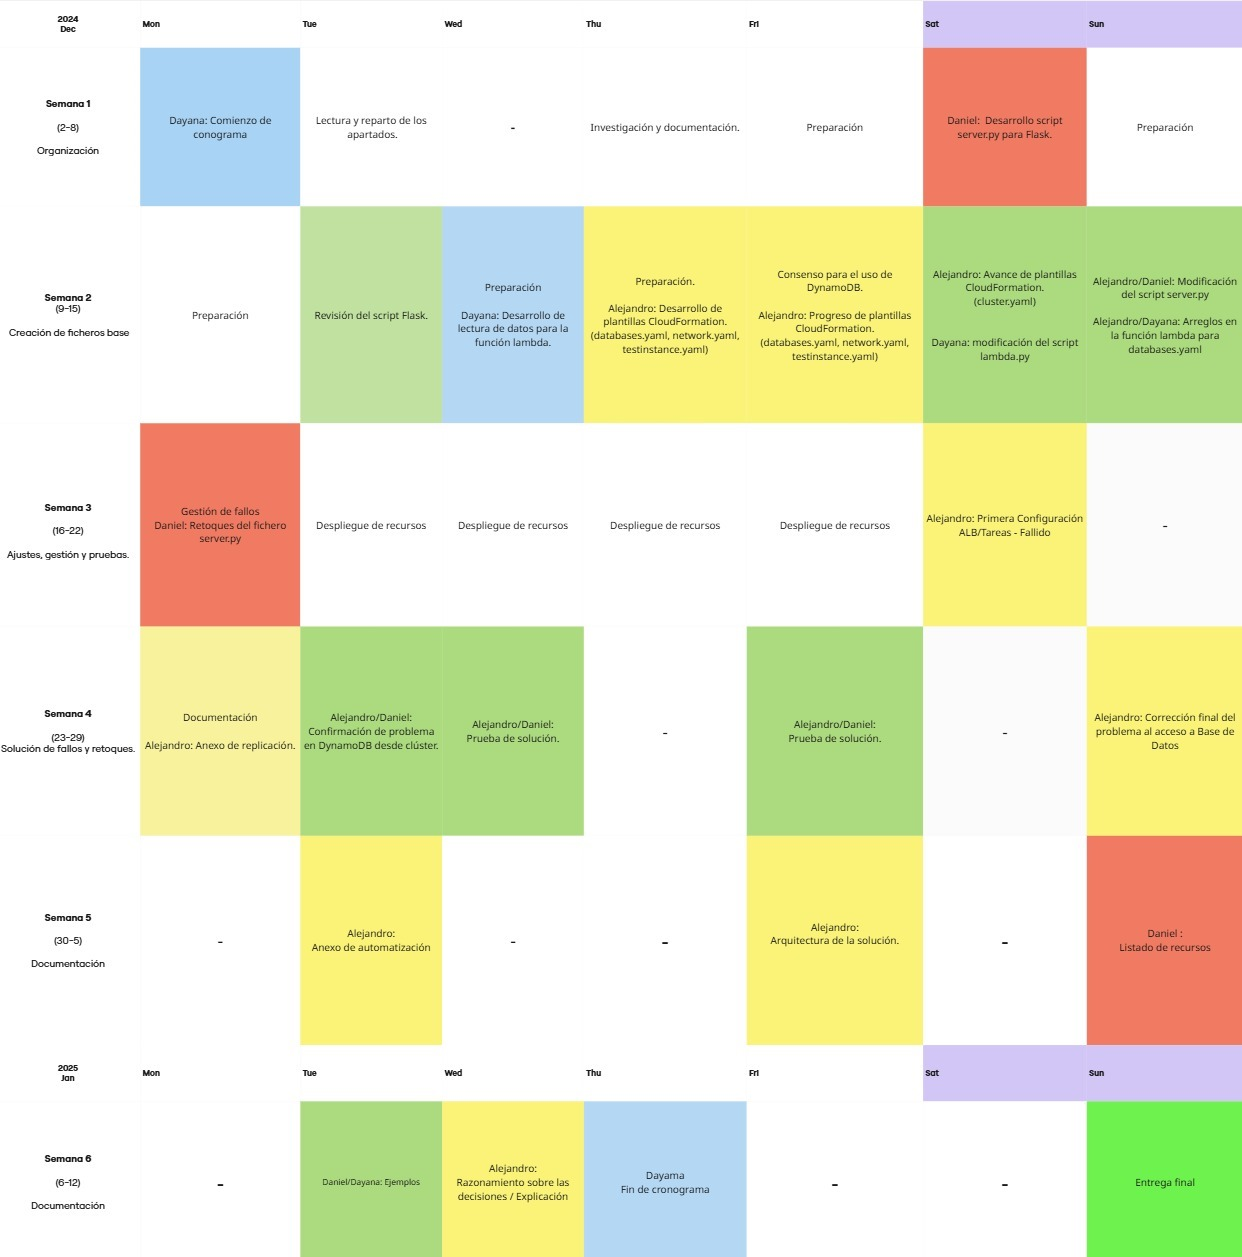
\includegraphics[width=\textwidth]{img/cronograma.jpeg}

\end{center}
